\chapter{Álcoois e fenóis}
\begin{mdframed}[backgroundcolor=orange!20,linewidth=0pt,roundcorner=10pt]
	\minitoc
\end{mdframed}
Após analisar funções orgânicas contendo apenas Carbono e Hidrogênio em suas moléculas, focamos nossa atenção em funções contendo o grupo \textbf{hidroxil} (OH) ligado a dois tipos de átomos de Carbono, o que origina duas funções distintas: \textbf{álcoois} (grupo hidroxil ligado a carbono saturado) e \textbf{fenóis} (grupo hidroxil ligado a carbono aromático), conforme pode ser visto na figura \ref{fig:af}

\begin{figure}[H]
	\centering
	\caption{Exemplo de substância da função álcool (glicerol) e de substância da função fenol (hidroquinona). Os nomes citados são \textbf{usuais}.}
	\vspace{0.5cm}
	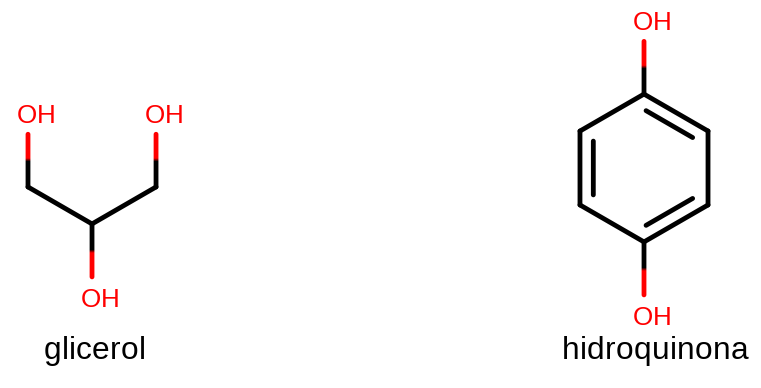
\includegraphics[width=0.7\linewidth]{imagens/af.png}
	\label{fig:af}
\end{figure}


Estas funções são bastante versáteis quando de trata de síntese orgânica, ou seja, reações orgânicas que permitem a obtenção de medicamentos, corantes, plásticos, entre muitas outras classes de substâncias orgânicas, o que lhes confere importância econômica quando pensamos em atividades industriais.

\section{Aspectos estruturais}
Podemos representar, de modo genérico, um álcool pela fórmula geral R-OH, onde R é um radical alquil (metil, etil, isopropil, entre outros) enquanto um fenol é representado pela fórmula geral ArOH, onde Ar é um radical aril (aromático), como fenil, naftil, entre outros.

Em termos estruturais, álcoois e fenóis são, simultaneamente, semelhantes e distintos, pois a presença do grupo OH ligado diretamente a um carbono saturado (álcoois) ou diretamente a um carbono aromático (fenóis) confere propriedades e reatividades distintas às duas funções.

Álcoois apresentam uma característica estrutural muito importante e que ajuda a explicar boa parte de suas propriedades: a possibilidade de formaçào de ligações de hidrogênio com água. A figura \ref{fig:ligacaoh}  ilustra a formação dessa ligação entre etanol (esquerda) e água (direita), \textbf{indicada pelo tracejado entre as duas moléculas}. Nesta representação, o átomo de carbono é a bola de cor cinza (maior), o hidrogênio é a bola branca (menor) e o átomo de oxigênio é a bola vermelha (tamanho intermediário).

 \begin{figure}[h]
	\centering
	\caption{Ligação de hidrogênio entre etanol e água, desenhada usando o software Avogadro \cite{avogadro}}
	\vspace{0.5cm}
	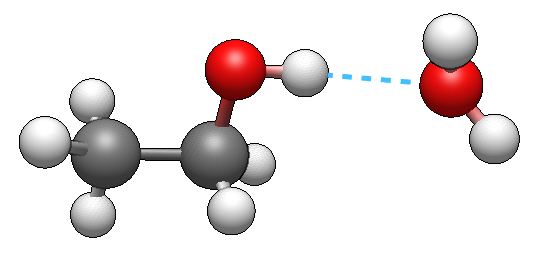
\includegraphics[width=0.65\linewidth]{imagens/ligacaoh.png}
	\label{fig:ligacaoh}
\end{figure}

\subsection{Caráter ácido/base}

Isoladamente, as moléculas de propanol e de fenol, usadas adiante como exemplo, são analisadas sem a presença de água ou qualquer outro solvente, apenas para ilustrar os efeitos decorrentes da presença do grupo OH nas duas funções. Por uma questão de simplicidade, usaremos apenas a propriedade periódica conhecida como \textbf{eletronegatividade}, juntamente com a \textbf{ressonância}, discutida anteriormente, para explicar as diferenças no caráter ácido/base do etanol e do fenol.

Parte da análise feita nesta seção utiliza o conceito de \textbf{pKa}, uma medida da ionização de uma substância quando encontra-se em solução aquosa.

A definição conceitual de pKa é a constante de equilíbrio de ionização de um ácido fraco, é uma medida da força de um ácido fraco. Quanto menor o pKa, mais forte é o ácido. Em termos mais simples, o pKa é o pH em que a concentração de ácido não ionizado é igual à concentração de ácido ionizado.

Por exemplo, o ácido acético, exibido na figura \ref{fig:ionizacao}, presenta valor de pKa igual a 4,76. Isso significa que, em uma solução aquosa com pH de 4,76, a concentração de ácido acético não ionizado é igual à concentração de ácido acético ionizado. Em pHs mais baixos, o ácido acético está mais protonado, ou seja, na forma de ácido. Em pHs mais altos, o ácido acético está mais desprotonado, ou seja, na forma de base.

\begin{figure}[h]
\centering
\caption{Exemplo da ionização de um ácido fraco}
\vspace{0.25cm}
\label{fig:ionizacao}
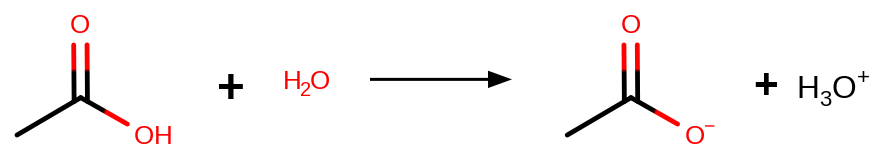
\includegraphics[width=0.9\linewidth]{imagens/ionizacao.png}
\caption*{Fonte: Autores}
\end{figure}

Matematicamente, temos:
\begin{equation}
	pK_ a = -log(K_ a)
\end{equation}

onde Ka é o valor da constante de equilíbrio de ionização do ácido acético:
\begin{equation}
	K_a = \frac{{\left[ {H_3O^ + } \right]\left[ {Ac^ - } \right]}}{{\left[ {HAc} \right]}}
	\label{eq:ionizacao}
\end{equation}

É importante notar, observando a equação \ref{eq:ionizacao}, que a quantidade em mol de água é muitísimo maior que todos os demais componentes do equilíbrio químico e está associada com K$_a$.

O átomo de oxigênio do grupo OH, nas duas funções aqui analisadas, encontra-se inicialmente com hibridização sp{$^3$} e apresenta uma relativamente elevada densidade eletrônica na região do grupo OH, conforme por ser observado nas figuras \ref{fig:subfenol} e \ref{fig:subpropanol} a seguir, que ilustram os mapas de potencial eletrostáticos para o fenol e o propanol.

Um mapa de potencial eletrostático é uma ferramenta de muito valiosa para visualizar a distribuição de cargas elétricas em uma molécula, bem como eventuais propriedades decorrentes desta disribuição de cargas.

A criação de um mapa de potencial eletrostático é normalmente feita com ajuda de um programa de computador por causa da enorme quantidade de operações matemáticas que devem ser feitas para calcular a energia potencia eletrostática nos diversos pontos da molécula, usando métodos derivados da Equação de Schrödinger \cite{Schrodinger}.

A visualização do mapa de potencial eletrostático é feita usando, por exemplo, uma paleta ou espectro de cores, normalmente usando a cor vermelha para menor potencial eletrostático e azul para maior potencial eletrostático.

Analisando a figura  com mais detalhes, podemos perceber uma região de cor vermelha próxima ao átomo de Oxigênio da função fenol, o que indica densidade eletrônica mais alta naquela região, compatível com a espécie \textbf{fenolato} que se forma na ionização do fenol em água.

\begin{figure}[H]
	\caption{Mapas de potencial eletrostático para fenol (a) e propanol (b)}
	\subfigure[Fenol]{\label{fig:subfenol}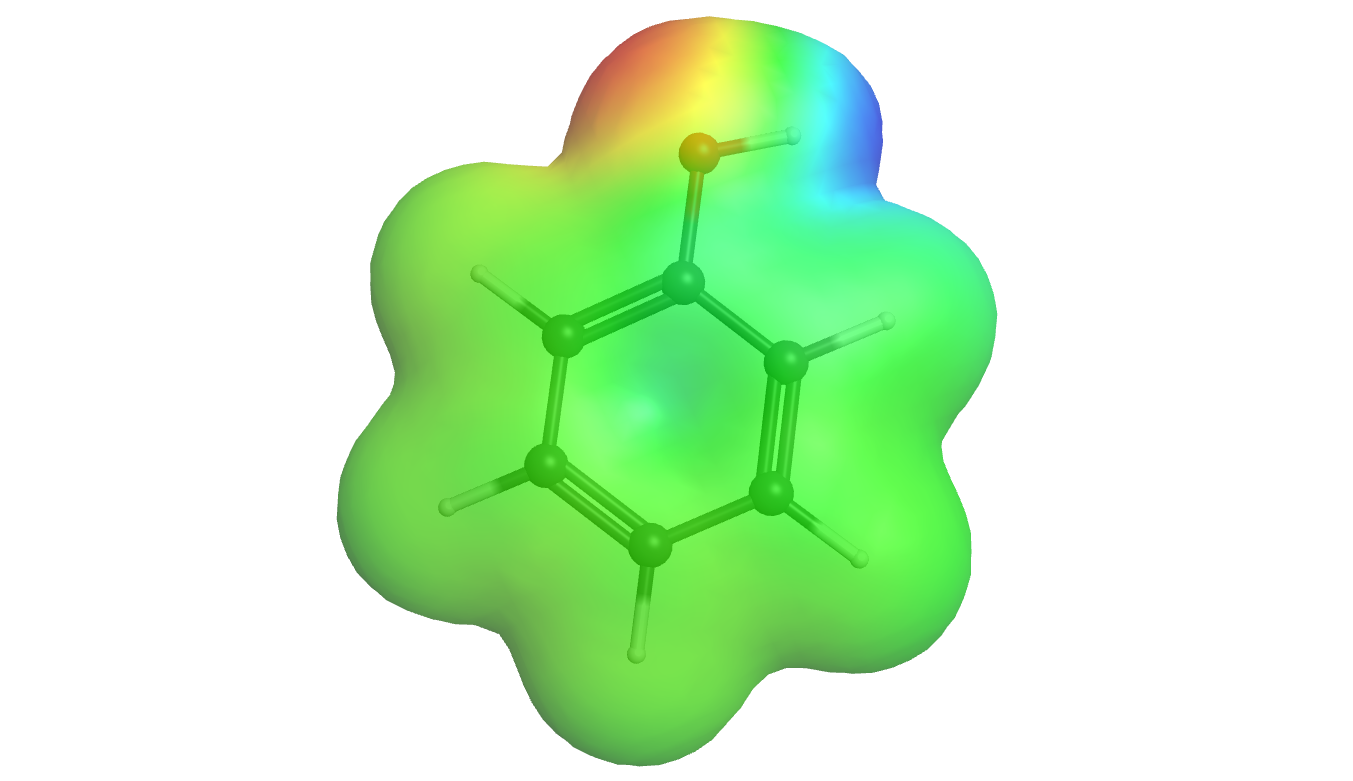
\includegraphics[width=90mm]{imagens/fenol.png}}
\hfill
	\subfigure[Propanol]{\label{fig:subpropanol}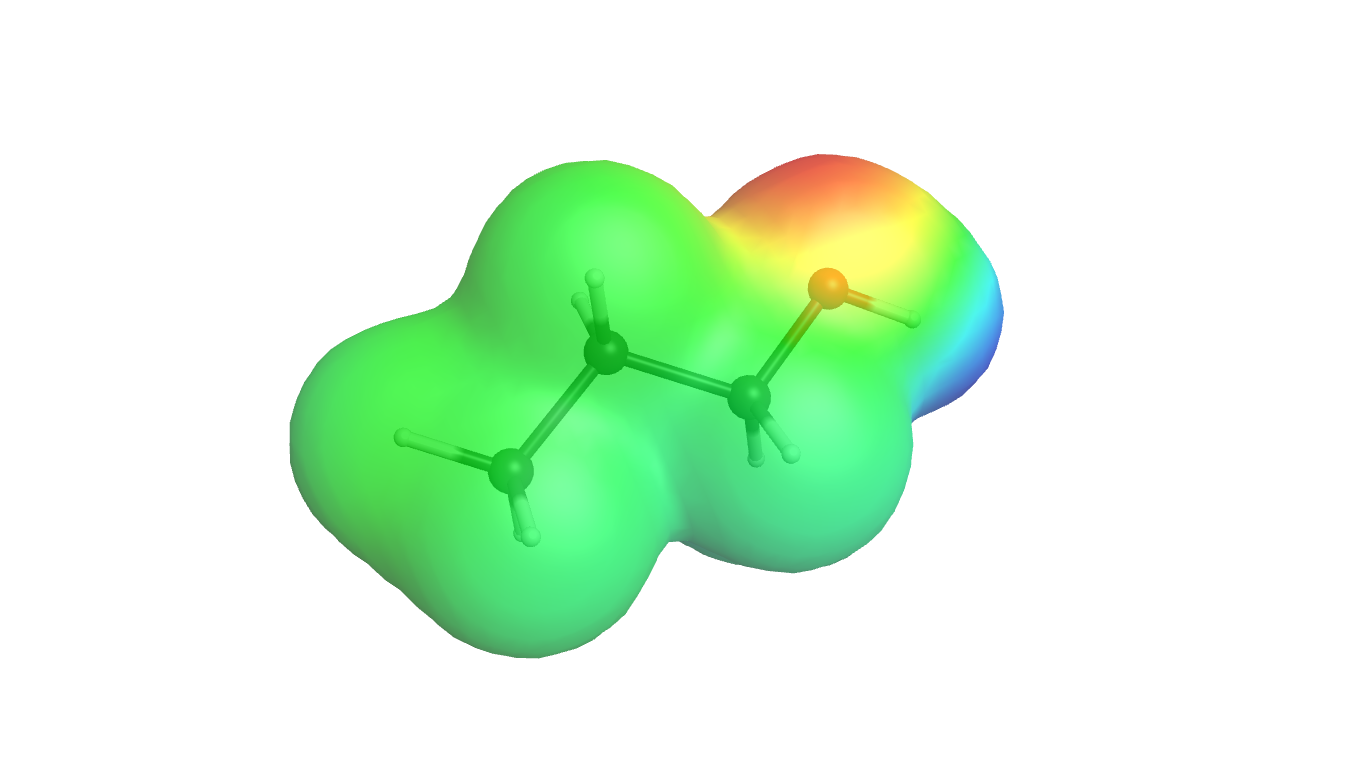
\includegraphics[width=90mm]{imagens/propanol.png}}
	\label{fig:subgraficos}
\end{figure}

A formação do íon fenolato em água ocorre através de um processo conhecido por ionização, ilustrado na figura \ref{fig:ionizacao}. Uma vez que a ligação H-O no fenol é bastante polarizada, conforme pode ser evidenciado no mapa de potencial eletrostático mostrado figura \ref{fig:subgraficos}, a quebra heterolítica da ligação H-O, provocada por ação da água, é facilitada.

O conceito de \textbf{ressonância} ajuda muito na compreensão do caráter ácido do fenol por causa da deslocalização da carga negativa do íon fenolato por meio do sistema aromático, conforme pode ser visto na figura \ref{fig:fenolfenolato}.

\begin{figure}[h]
\centering
\caption{Ionização do fenol, com estruturas de ressonância}
\vspace{0.5cm}
\label{fig:fenolfenolato}
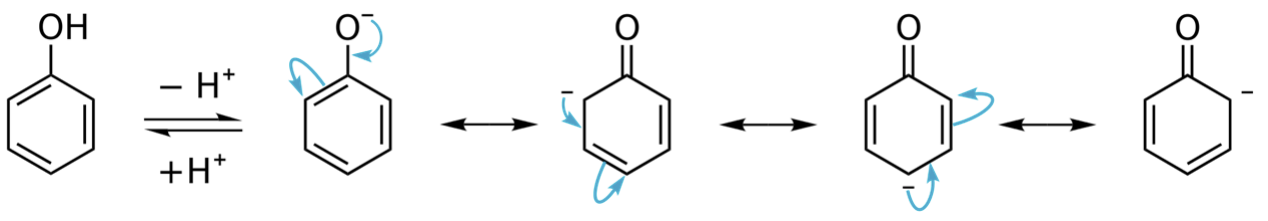
\includegraphics[width=1\linewidth]{imagens/fenolato.png}
\caption*{Fonte: Universidade de São Paulo, disponível em https://shorturl.at/fjrX8}
\end{figure}

A figura \ref{fig:fenolfenolato} esclarece as razões pelas quais o íon fenolato é estável e, portanto, o fenol apresenta caráter ácido. Da esquerda para a direita, temos o fenol perdendo um cátion H$^+$ por ionização em água e convertendo-se no íon fenolato, caracterizado por uma carga elétrica negativa no átomo de oxigênio. As setas indicam a movimentação dos elétrons no sistema conjugado do anel aromático, conforma descrito em -inserir refrência sobre ressonância-.
Repare que as ligações covalentes duplas tem suas posições alteradas por duas características peculiares do sistema aromático: \textbf{(a)} planaridade dos átomos do anel aromático e \textbf{(b)} presença de orbitais p puros, possibilitando a ressonância e a consequente deslocalização da carga negativa ao longo do ciclo aromático.

Comparado com o fenol (pK$_a$ = 10), etanol ou propanol (ambos com pK$_a$ = 16) \textbf{não possuem quaisquer resquisitos estruturais para estabilização da carga negativa} no átomo de Oxigênio e, portanto, não apresentam caráter ácido.

\subsection{Propriedades físicas}
Álcoois como metanol, etanol e propanol são totalmente solúveis em água por razões tratadas anteriormente, mas à medida em que aumenta o número de átomos de Carbono da cadeia, a solubilidade em água diminui em função do aumento da contribuição da cadeia carbônica, essencialmente apolar, minimizando a ação das ligações de hidrogênio possíveis entre o grupo hidroxil e água. Assim o butanol é menos solúvel em agua em relação aos álcoois de menor cadeia carbônica. Analisando a tabela \ref{solubilidade}, percebemos a influência da cadeia carbônica na solubilidade de alguns álcoois em dois solventes muito comuns: água (para substâncias polares) e hexano (para substâncias apolares). Cadeias carbônicas maiores fazem com que o álcool tenha solubilidade muito reduzida e comporte-se quase como um hidrocarboneto. Para que ocorra a dissolução do álcool, é necessário que as ligações de hidrogênio entre o álcool/água rompam as ligações de hidrogênio água/água, o que não ocorre em álcoois de cadeia carbôncia maior.

\begin{table}[!h]
	\begin{center}
	\caption{\label{solubilidade}Solubilidade de alguns álcoois em água e hexano (g/100g de solvente)\cite{solubilidade}}
	\vspace{0.5cm}
	\begin{tabular}{l c c}
	\hline
	Nome & Solubilidade em água & Solubilidade em hexano\\
	\hline
	Metanol & $\infty$ & 3,8\\
    %\hline
	Etanol & $\infty$ & $\infty$\\
	%\hline
    Propanol & $\infty$ & $\infty$\\
	Butanol & 7,9 & $\infty$\\
	Heptanol & 0,2 & $\infty$\\
    \hline
	\end{tabular}
	\end{center}
	\caption*{Fonte: referência \cite{solubilidade}}
\end{table}

Por outro lado, fenóis apresentam cadeia carbônica superior a vários álcoois e, portanto, possuem solubilidade menor, mas preciusamos considerar o efeito da ionizaçãod e fenóis em água, discutido anteriormente, e que ajuda a explicar a maior solubilidadede do, por exemplo, fenol comparado com um álcool de massa molar próxima, conforme pode ser visto na tabela \ref{comparada}.

\begin{table}[!h]
	\begin{center}
	\caption{\label{comparada}Solubilidade comparada do fenol e do pentanol}
	\vspace{0.5cm}
	\begin{tabular}{l c c c}
	\hline
	Nome & Massa molar (g/mol) &Solubilidade em água & Solubilidade em hexano\\
	\hline
	Fenol & 94 & 8,0 & 3,8\\
    %\hline
	Pentanol & 88 & 2,3 & $\infty$\\
	Hexanol & 102 & 0,6 & $\infty$\\
    \hline
	\end{tabular}
	\end{center}
	\caption*{Fonte: Autores}
\end{table}

O ponto de ebulição de álcoois varia de acordo com o tamanho da cadeia carbônica, como pode ser observado na figura \ref{fig:ebulicao}, e o ponto de ebulição de fenóis varia aproximadamente da mesma forma \cite{fisicas}.

\begin{figure}[h]
	\caption{Ponto de ebulição de alguns álcoois em função cadeia carbônica (\textcelsius)}
	\label{fig:ebulicao}
	
	\vspace{0.5cm}
	\centering
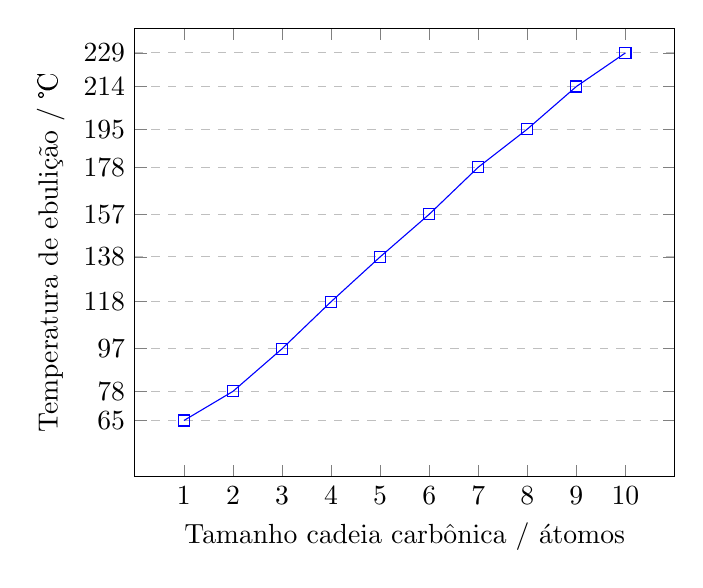
\begin{tikzpicture}
	\begin{axis}[
		title={},
		xlabel={Tamanho cadeia carbônica / átomos},
		ylabel={Temperatura de ebulição / \textcelsius},
		xmin=0, xmax=11,
		ymin=40, ymax=240,
		xtick={1,2,3,4,5,6,7,8,9,10},
		ytick={65,78,97,118,138,157,178,195,214,229},
		legend pos=north west,
		ymajorgrids=true,
		grid style=dashed,
	]
	\addplot[
		color=blue,
		mark=square,]
		coordinates {(1,65)(2,78)(3,97)(4,118)(5,138)(6,157)(7,178)(8,195)(9,214)(10,229)};
		\legend{}
	\end{axis}
\end{tikzpicture}
	\caption*{Fonte: Autores}
\end{figure}

%\section{Obtenção e usos}
\section{Ocorrência e aplicações}
Conforme já mencionado no início deste capítulo, álcoois e fenóis são compostos versáteis e muito úteis em diversos setores econômicos e industriais, e considerando o etanol como um dos protagonistas, por suas aplicações variando de componente de bebidas até combustíveis automotivos, passando por produtos de limpeza, tanto domésticos quanto hospitalares.

\subsection{Álcoois}
Muitos exemplos de substâncias pertencentes à função álcool possuem usos biológicos e/ou aplicações industriais e podemos fixar nossa análise em compostos monofuncionais, ou seja, possuem apenas a função álcool.

\subsubsection{Metanol}
Assim, o mais simples dos álcoois, o composto de fórmula \ce{CH3OH} recebe o nome de metanol, pois possui apenas um carbono e o hidreto pai é o metano. Pela nomenclatura substitutiva, um átomo de Hidrogênio foi substituído pelo grupo OH e álcoois possuem o sufixo ol. Justificado o nome \textbf{metanol}, certo?

\begin{figure}[h]
    \centering
    \caption{Fórmula estrutural para o metanol}
    \vspace{0.5cm}
    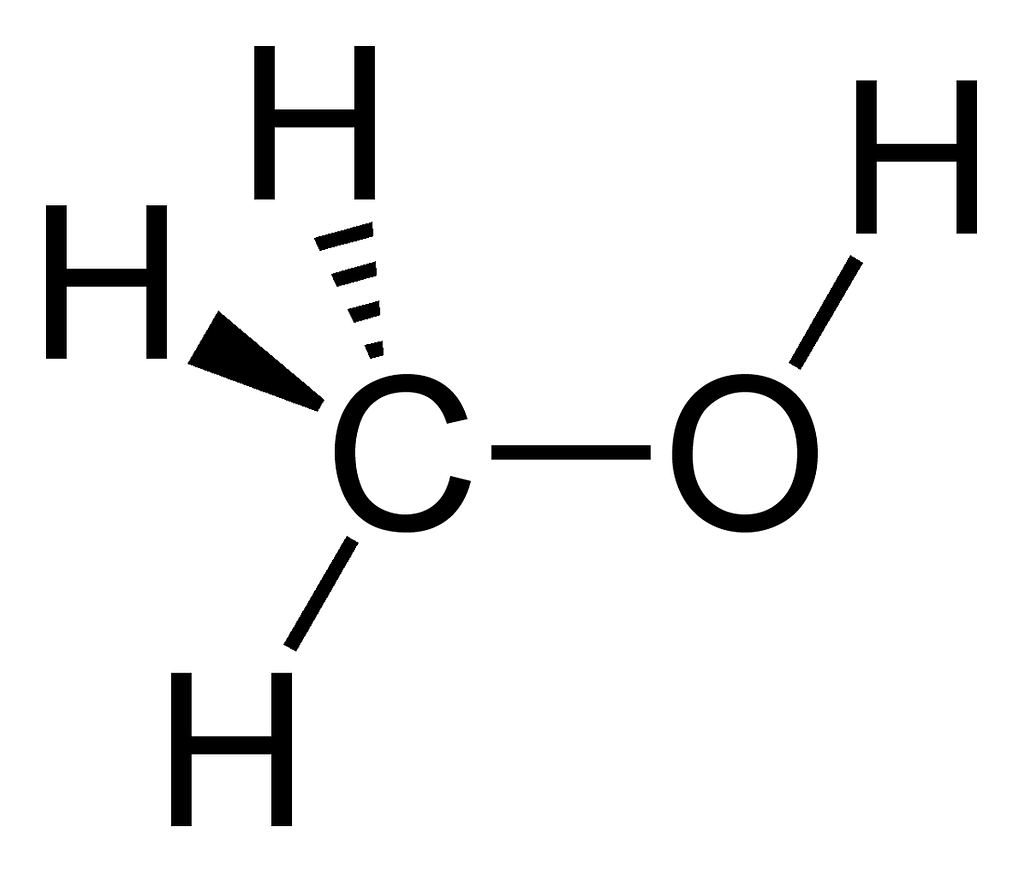
\includegraphics[width=0.2\linewidth]{imagens/methanol-2d-0349e4-1024.png}
\label{fig:mpemetanol}
\end{figure}

A figura \ref{fig:mpemetanol} a seguir ilustra o mapa de potencial eletrostático para o metanol e tal mapa indica a distribuição de cargas elétricas na substância, utilizando uma paleta de cores que vai do azul ao vermelho, onde este último indica maior quantidade de carga em uma dada região, comparada com a cor azul de outra região.

\begin{figure}[h]
    \centering
    \caption{Mapa de potencial eletrostático para o metanol}
    \vspace{0.5cm}
    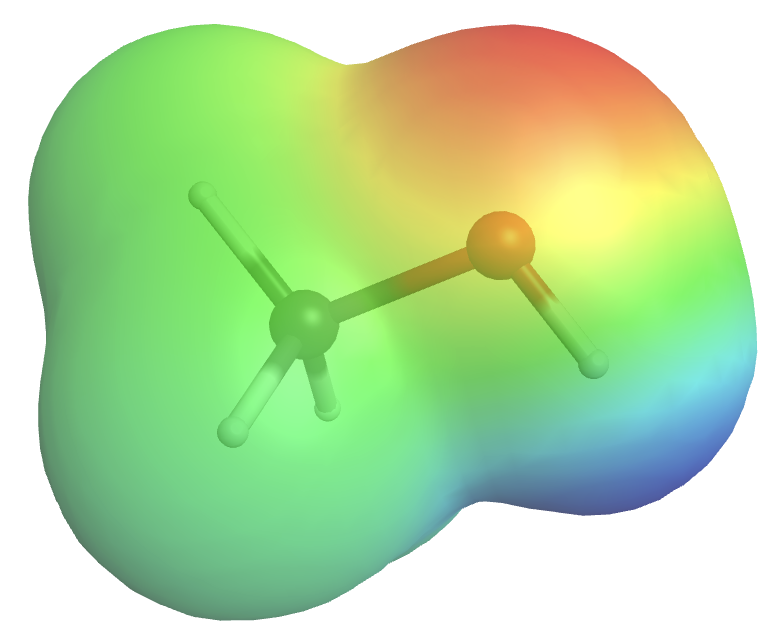
\includegraphics[width=0.45\linewidth]{imagens/mpemetanol.png}
\label{fig:mpemetanol}
\end{figure}

Um estudo recente realizado no Brasil \cite{D2CC01757A} mostra a foto-oxidação de metano para produzir metanol em condições ambientes, catalisada por metais de transição. Comparado com métodos clássicos, as condições reacionais e a possibilidade de uso de luz solar no processo tornam esse estudo muito promissor na produção em escala industrial de metanol.

A toxicidade do metanol, indicada pelo Diagrama de Hommel, indicado na figura \ref{fig:hommel} a seguir, pode ser analisada considerando as quatro partes da imagem contendo números inteiros em uma escala entre 0 e 4, onde 0 indica ausência de problemas e 4 indica perigo crítico.

A figura geométrica do losango é usada pela NFPA (National Fire Protection Association) \footnote{Veja mais em https://www.nfpa.org/codes-and-standards/7/0/4/704}, nos Estados Unidos da América, para indicar riscos associados a cada substância cadastrada na instituição.

A parte em cor vermelha (porção superior do losango) indica a \textbf{inflamabilidade} da substância, ou seja, sua capacidade de entrar em combustão. Portanto, o metanol é bastante inflamável e com um seríssimo agravante: sua combustão gera chamas de cor azul muito claras e visíveis apenas à noite, exigindo mais cuidados em sua manipulação. Diversos acidentes envolvendo metanol já foram citados e aqueles envolvendo automóveis de corrida da chamada Fórmula Indy, categoria automobilística muito famosa nos Estados Unidos da América, são chocantes \footnote{Veja mais em https://www.essentiallysports.com/nascar-news-invisible-fire-at-the-nineteen-eighty-one-indy-five-hundred-sets-the-nascar-community-ablaze-after-fans-make-talladega-superspeedway-nights-connection/}.

A parte em cor azul (porção central e esquerda do losango) indica o \textbf{risco à saúde} e, portanto, o contato ou ingestão deve ser evitado. Para referência, a dose letal por via oral em ratos é de pouco mais de 5,6 g/kg de peso corporal.

A parte em cor amarela (porção central direita do losango) indica \textbf{instabilidade ou reatividade} e mostra a estabilidade do metanol.

A parte em cor branca (porção inferior do losango) indica \textbf{risco específico} (oxidante forte ou radioativo, por exemplo) e não há registros de tal categoria para o metanol.


\begin{figure}[h]
    \centering
    \caption{Diagrama de Hommel para o metanol}
    \vspace{0.5cm}
    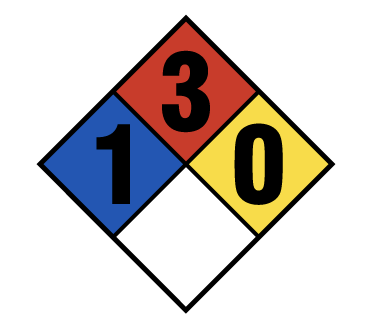
\includegraphics[width=0.25\linewidth]{imagens/hommel.png}
\label{fig:hommel}
\end{figure}

\subsubsection{Etanol}
Este álcool possui tamanha importância no Brasil, seja como combustível, como componente de produtos de limpeza ou em bebidas alcoólicas, que seu nome se confunde com a função orgânica à qual pertence \cite{raizen}. Por muito tempo os brasileiros compravam "álcool" em postos de combustíveis e apenas recentemente a substância passa a ser comercializada com seu nome oficial.

Trata-se de um líquido transparente, incolor, com densidade em torno de 0,8 g/cm$^3$ e miscível com água em qualquer proporção, explicado por meio da formação de ligações de hidrogênio entre água e etanol de modo tão intenso, que a mistura líquida é classificada como azeótropo, ou seja, os componentes da mistura entram em ebulição juntos, o que inviabiliza a destilação comum como meio de separação dos componentes desta mistura. Porém, é possível separar os componentes da mistura por outros métodos \cite{trica}.

\begin{figure}[h]
	\centering
	\caption{Diferentes representações para o etanol}
	\vspace{0.5cm}
	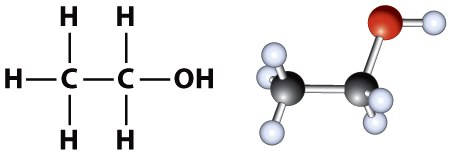
\includegraphics[width=0.75\linewidth]{imagens/etanol2.jpeg}
	\label{fig:etanol2}
\end{figure}

A figura \ref{fig:etanol2} ilustra ao menos duas representações distintas para o etanol: a fórmula estrutural completa (esquerda) e a representação do tipo "ball \& stick" (tubo e bola) (direita), onde as bolinhas de cores e/ou tamanhos diferentes representam os átomos e os tubinhos representam as ligações químicas entre eles. Existem diferentes representações para moléculas orgânicas em função do contexto de uso, onde uma dada representação pode ser mais esclarecedora que outra.

No Brasil, o etanol é produzido, essencialmente, por fermentação de sacarose por meio de leveduras, em inúmeras usinas de produção espalhadas pelo país, fato que movimenta um enorme número de trabalhadores nos diversos segmentos de produção e distribuição, alimentando uma cadeia produtiva bastante ampla.

Como é produzido a partir da sacarose obtida pela cana-de-açúcar, parte do dióxido de carbono, CO$_2$, produzido pela queima do etanol em motores a combustão, podemos dizer que o etanol é um combustível de ciclo neutro, conforme pode ser visto na figura \ref{fig:neutro} a seguir. Por "combustível de ciclo neutro", entenda, no caso do etanol, que sua principal fonte de obtenção é a cana-de-açúcar, vegetal com folhas verdes e capaz de realizar fotossíntese. Assim, a planta que origina o etanol captura parte das moléculas de CO$_2$ da atmosfera (algumas destas provenientes do etanol) e diminui os efeitos ambientais causados pela combustão do etanol como biocombustível.

\begin{tcolorbox}[colback=white!5!white,colframe=orange!90!black,title=\textbf{Equações de combustão do etanol (linha 1) e gasolina (linha 2)}]
	\ce{C2H6O + 3 O2 -> 2 CO2 + 3 H2O}
	\tcblower
	\ce{C8H18 + 25/2 O2 -> 8 CO2 + 9 H2O}
	\vspace{0.5cm}
	
	Consideramos o \ce{C8H18} como o principal componente da mistura comercial chamada \textbf{gasolina}.
\end{tcolorbox}

Em comparação, a gasolina, outro combustível muito importante na matriz energética brasileira, não possui qualquer elemento em sua origem capaz de absorver o CO$_2$ liberado em sua queima, uma vez que trata-se de um combustível de origem fóssil. Portanto, a gasolina é mais poluente que o etanol. Ainda, a combustão da gasolina libera muito mais moléculas de CO$_2$ na atmosfera, por mol de combustível utilizado, que a combustão do etanol, e nesta análise não consideramos eficiência energética ou o antigo conceito de poder calorífico.

 \begin{figure}[h]
 	\centering
 	\caption{Etanol como combustível de ciclo neutro}
 	\vspace{0.5cm}
 	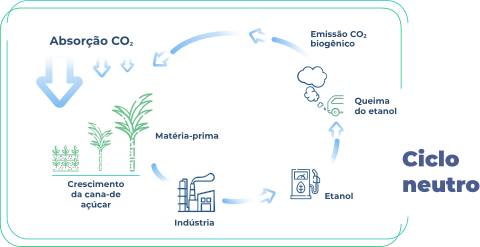
\includegraphics[width=0.75\linewidth]{imagens/ciclo-neutro.png}
 	\label{fig:neutro}
 \end{figure}

 \subsection{Fenóis}
Seres humanos convivem com fenóis há séculos, desde a Mesopotâmia, e o consumo de substâncias derivadas de plantas para os mais diversos fins incluem fenóis, simples, ácidos fenólicos \footnote{Compostos fenólicos contendo ao menos um grupo carboxil, -COOH}, flavonóides, cumarinas entre muitas outras classes de compostos fenólicos. A figura \ref{fig:fenolicos} a seguir ilustra alguns destes ácidos fenólicos \cite{fenolicos}. Muitos destes fenóis são considerados agentes importantes nos mecanismos de curas de doenças.

Ácidos fenólicos também estão envolvidos na proteção contra patologias cardiovasculares, câncer, diabetes, processos inflamatórios, entre muitos outros \cite{robbins2003phenolic}.

Diabete mellitus é identificada como uma desordem de stress oxidativo, como consequência do desequilíbrio entre a formação de radicais livres em uma pessoa e sua capacidade de os oxidar. Existe uma bem conhecida relação entre obseidade e diabetes e o consumo regular de compostos fenólicos pode ajduar a prevenir e/ou controlar esse tão grave problema de saúde pública mundial \cite{furukawa114nakayama}.

Câncer é um dos maiores problemas de saúde pública mundial e os riscos de desenvolver essa patologia podem ser diminuídos pelo consumo de alguns anti-oxidantes contendo ácidos fenólicos \cite{kumar2017quantum}.

Ácidos fenólicos são disponíveis comercialmente como suplementos alimentares, contendo aotni-oxidantes e são rapidamente absorvidos pelo organismo humano, resultando em alta biodisponiblidade.

\begin{figure}[h]
	\centering
	\caption{Exemplos de ácidos fenólicos. O ácido cinâmico, extraído do óleo de canela, é utilizado na indústria de perfumes e também como fungicida. O ácido gálico é um bem conhecido anti-oxidante natural, um metabólito secundário, aquele produzido a partir dos metabólitos primários, como carboidrados, aminácidos e lipídeos.}
	\vspace{0.5cm}
	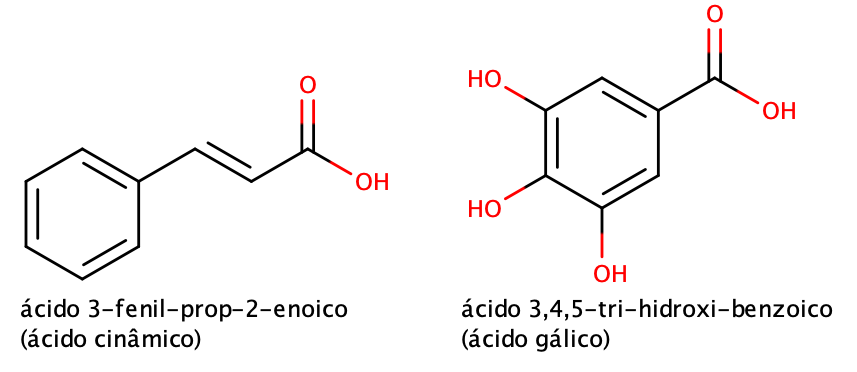
\includegraphics[width=0.75\linewidth]{imagens/acidosfenolicos.png}
	\label{fig:fenolicos}
	%\caption*{Fonte: Autores}
\end{figure}
